This chapter explores the requirements of a digital back-end suited to a Q-Pix based readout implemented in a LArTPC design at DUNE-FD scales.

The first part of this chapter describes the simulation methodology used to evaluate the possible designs presented in the previous chapter.
The Q-Pix readout~(Chapter~\ref{chap:qpix}) relies on several key factors which promise possible improvements over a traditional MWPC readout: automatic calibration from quesicent background, an overall reduction in data collection, and simpler analysis chain and vertex reconstruction, to name a few.
However, this novel readout technique not only changes the front-end analog structure but also dramatically increases the number of digitization channels.
The increase of the number digital channels and required ASICs creates the need for a new digital-backend design.

The second part of this chapter presents results from the simulation framework which parameterizes the search for an optimal digital design.
We use this simulation framework to address these questions, since any sufficiently complicated design offers an intractible number of possible choices each of which can signficantly alters the performance (good or bad) of a detector.
The Q-Pix readout is no different.
A few examples of crucial design choices for the digital back-end are: the use of free-running local oscillators, the selection of an inter-ASIC communication protocol, the choice of inter-ASIC connections or routing profiles, and the buffer sizes of FIFOs to store charge-reset data.
The goal of the simulation is to parameterize these design choices.

The final part of this chapter synthesizes the results of the simulations and provides, to the best of its ability, a description of the effects of the most important parameters determined from these results.
We use as inputs to the simulation the expected input charge from radiogenic background and beamline neutrino interaction over a DUNE-FD APA.
The characterization of the analog front-end, namely the charge characteristics per channel is an on-going collaborative work, whose results (when available) should be able to be applied here.
The goal of the next chapter~\ref{chap:qdb.tex} is to provide a hardware verification of the simulation results presented here.

All results from simulation in this chapter, with the exception of Section~\ref{sec:supernova} is my own individual work.

\section{The Tile Simulation Framework}

The previous chapter introduced the digital backend as well as discussed different design choices, namely tile size, routing configurations, and the effects of Aggregator position.
Here we describe how we simulate events of interested for these different tile configurations.

A successful design is able to record and send loss-less data for all events of interest.
In a DUNE-FD LArTPC these sources range in intensity from sub-MeV-scale radiogenic backgrounds native to the LAr to 10's of GeV scale of beam neutrinos or atmospheric neutrinos.
we consider the back-end design to be successful if and only if it provides the ability to fully capture and tramsit of all RTDs from these sources.

%%% Example of Digital Neutrino Events
\begin{figure*}
  \centering
  \begin{subfigure}[b]{0.475\textwidth}
      \centering
      \includegraphics[width=\textwidth]{./images/example_16_local_stack_slow.pdf}
      \caption[Network2]%
      {{\small Network 1}}    
  \end{subfigure}
  \hfill
  \begin{subfigure}[b]{0.475\textwidth}  
      \centering 
      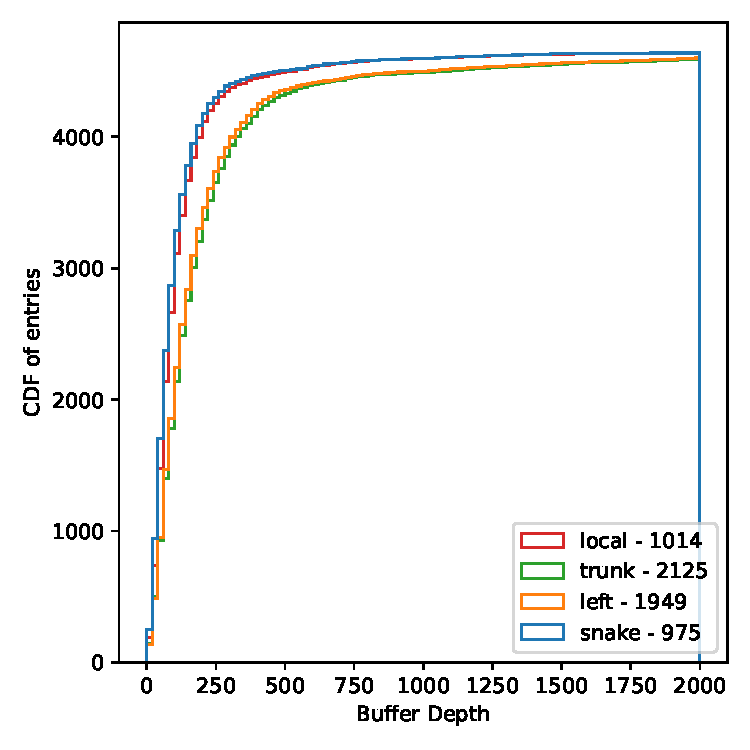
\includegraphics[width=\textwidth]{./images/example_16_remote_stack_slow.pdf}
      \caption[]%
      {{\small remote stack}}    
  \end{subfigure}
  \vskip\baselineskip
  \begin{subfigure}[b]{0.475\textwidth}   
      \centering 
      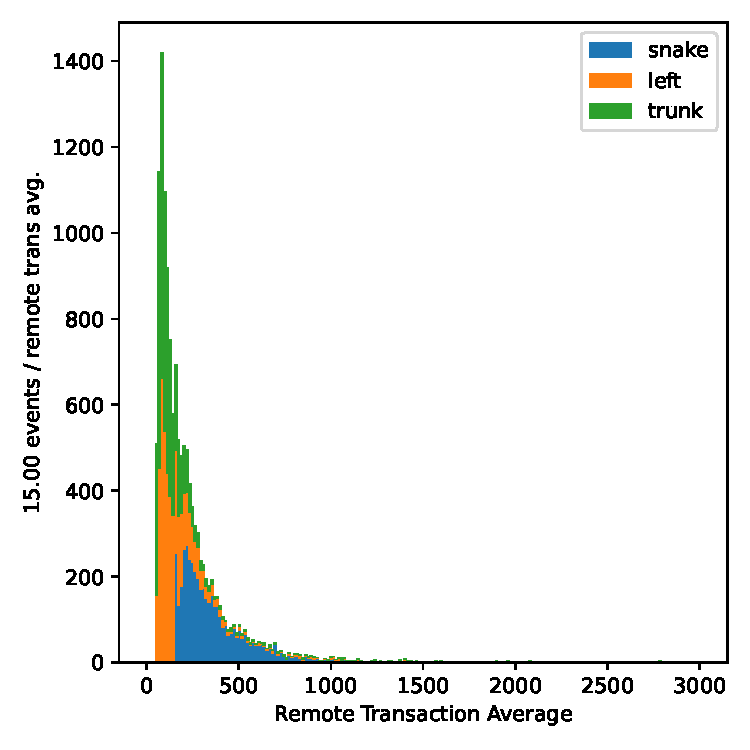
\includegraphics[width=\textwidth]{./images/example_16_remote_transact_slow.pdf}
      \caption[]%
      {{\small transact}}    
  \end{subfigure}
  \hfill
  \begin{subfigure}[b]{0.475\textwidth}   
      \centering 
      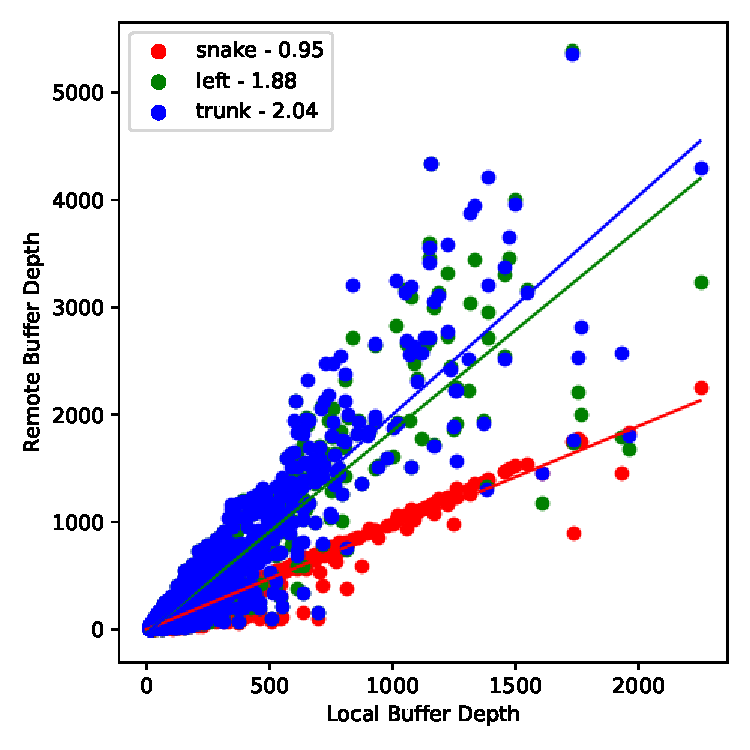
\includegraphics[width=\textwidth]{./images/example_16_route_fits_slow.pdf}
      \caption[]%
      {{\small route fits}}    
  \end{subfigure}
  \caption[ Information on the 4 by 4 tile. ]
  {\small all of the data } 
  \label{fig:example_plots_for_digital_sim}
\end{figure*}

\subsection{Tile Parameters}

\begin{table}
\begin{center}
\begin{tabular}{|| p{30mm} | p{30mm} | p{90mm} ||}
 \hline
 Name & Values & Relation \\ [0.5ex]
 \hline\hline
  Frequency Drift & 1\%, 5\% & Packet buildup within the tile \\
 \hline
  Tile Size & 4x4, 8x8, 10x14, 16x16 & Affects total number of resets which must be routed to aggregator.\\
 \hline
  Routing & Snake, Left, and Trunk & Different trees affect packet buildup as well as transaction count  \\
 \hline
  Architecture & Push, Pull & Describes conditions for when node enters transmit-local state.~\ref{sec:local_data_packet}  \\
 \hline
\end{tabular}
\caption{The different tile parameters that are used for the effective tile search.
  The frequency drift relates the relative distribution of the frequency of adjacent oscillators.
  The tile size determines how many digital nodes are within a single tile.
  The routing configurations are described in detail in the previous chapter, and refer to how local data words are sent to the aggregator.
  The two different architectures define how the node enters the transmit local state.
  The push architecture enters whenever a new reset is acquired, whereas the pull architecture enters only when a data request is received from the aggregator.}
\end{center}
\end{table}
~\label{table:tile_params}

\subsection{Tile Events}

\begin{figure}[]
\centering
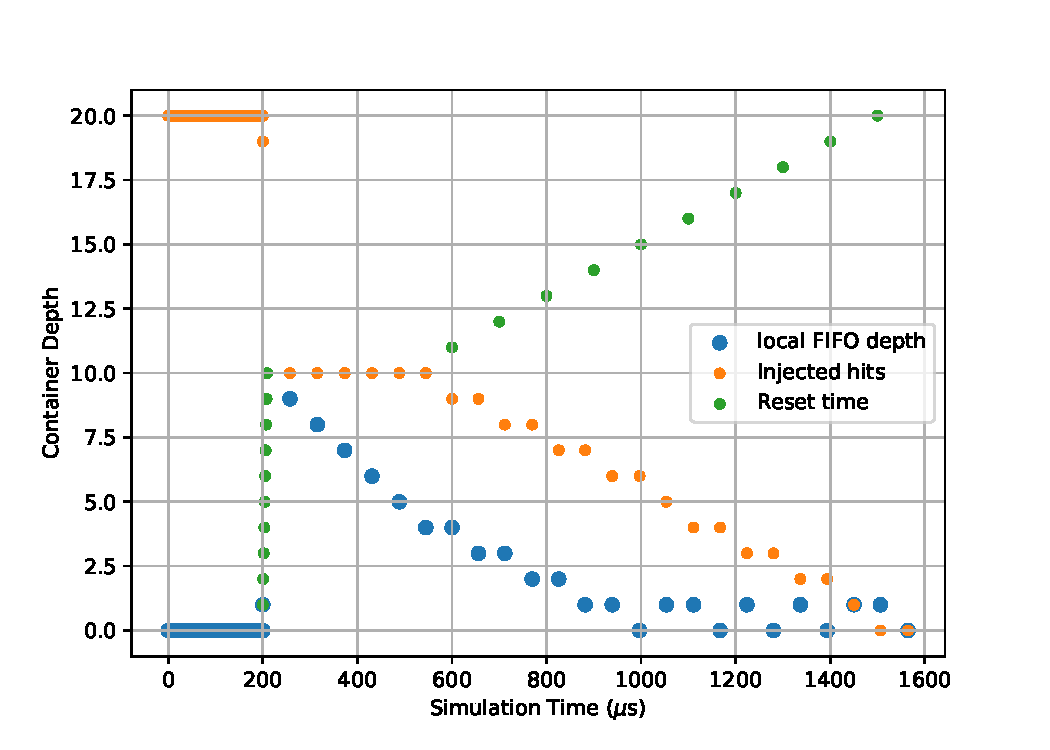
\includegraphics[width=\textwidth]{images/push_arch_buff.pdf}
\caption{A simulated push Architecture with injected hits.}
\end{figure}~\label{fig:push_arch_verification}

\begin{figure}[]
\centering
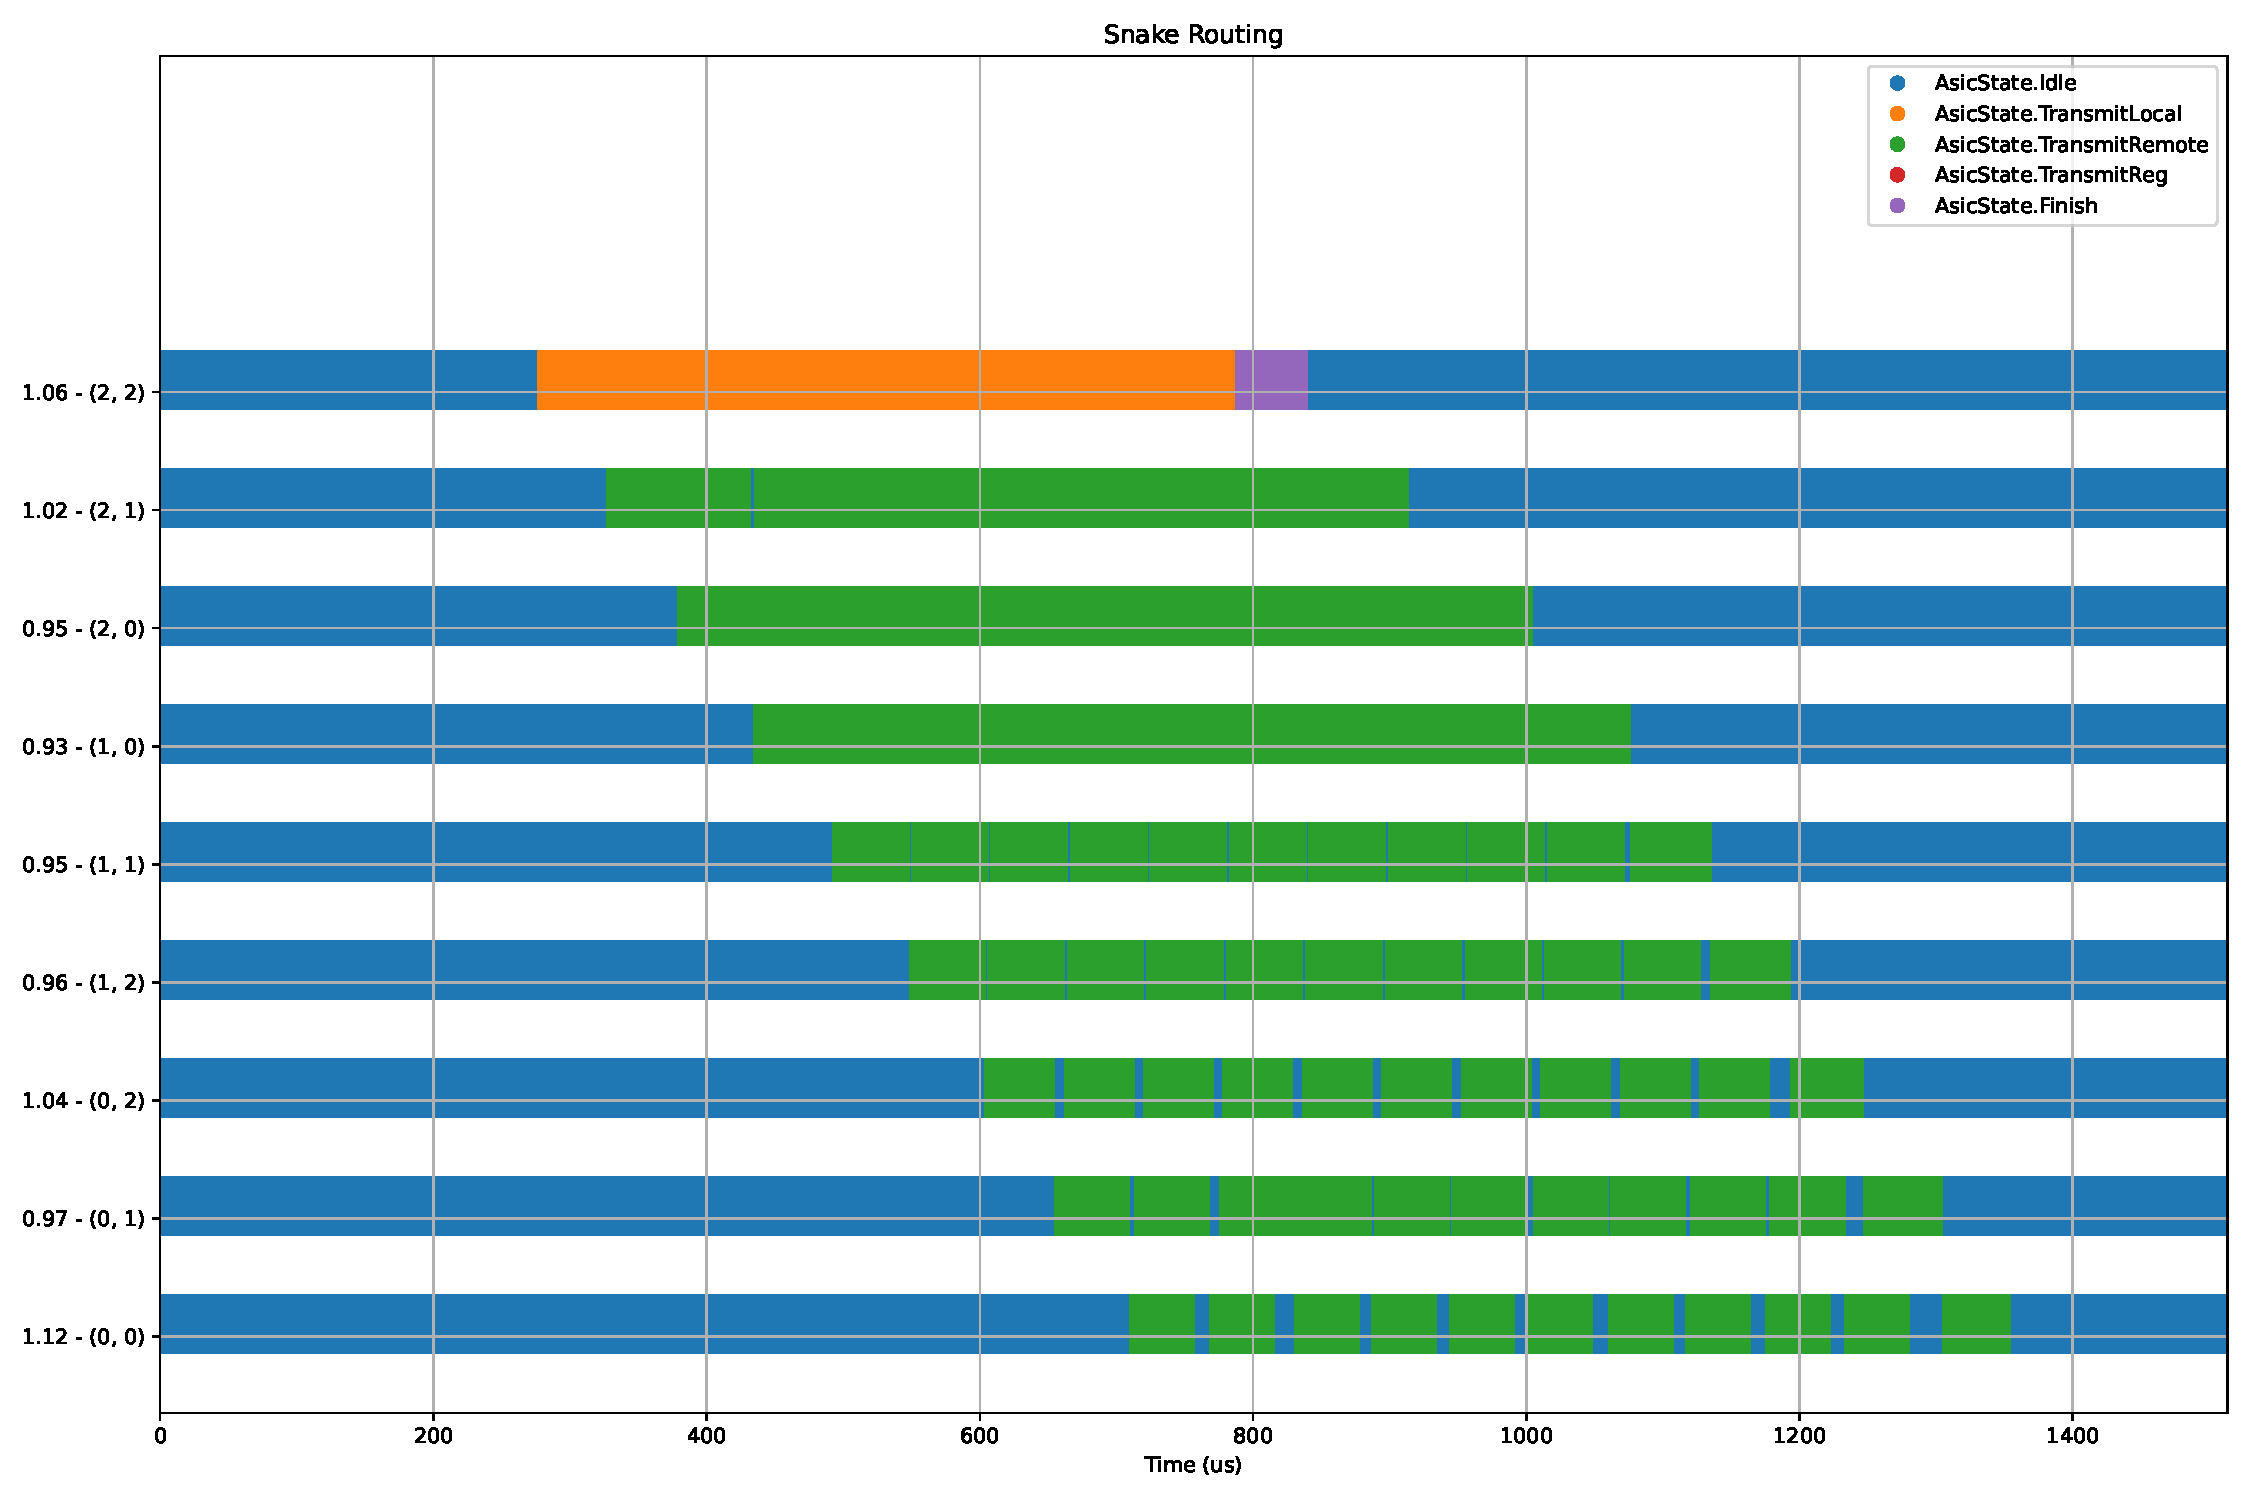
\includegraphics[width=\textwidth]{images/snake_timer.pdf}
\caption{Example of packet drift in the simulation framework.
  Packets drift apart in time as they are sent from slower to faster ASICs.
  Therefore, there is a possiblity of packet drift and asynchronous packet sending which depends on the magnitude of the frequency drift between neighbor ASICs.}
\end{figure}~\label{fig:packet_drift}

\begin{figure}[]
\centering
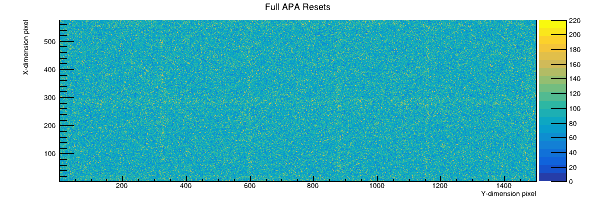
\includegraphics[width=\textwidth]{images/fullApaResets.png}
\caption{Full 1000s radiogenic background source simulation input into all pixels.}
\end{figure}~\label{fig:background_simulation}


\section{Physical Simulation Studies}
%% TODO - channel level heatmap for neutrino event

We now discuss the implementation of the simulation based on the previous sections.

\subsection{Simulated Detector Properties}



%%
\subsection{Radiogenic Backgrounds as a Calibration Source}

sources of backgrounds are taken from~\citep{DUNE-FD_TDRv4:Abi_2020}
Radiological Backgrounds~\citep{ar39_backgrounds, phd_backgrounds}

%% list of sources here
We use the following list of radiogenic sources of 10 separate iterations of runs of 1000 seconds.

\begin{table}
\begin{center}
\begin{tabular}{|c c c c c c|}
 \hline
 Isotope & Rate [Bq/kg] & Region & Region Mass [kg] & Rate [Bq] & Number of Decays (per 10 s window) \\ [0.5ex]
 \hline\hline
  $^{210}$Po & 0.2 & PD [Bq/$m^2$] & 2.46856 & 0.493712 & 5 \\
  $^{60}$Co & 0.0455 & CPA & 90 & 4.095 & 41 \\
  $^{40}$K & 0.49 & APA & 258 & 1,264.2 & 12,642 \\
  $^{39}$Ar & 1.010 & bulk LAr & ~70,000 & 70,700 & 707,000 \\
  $^{42}$Ar & 0.000092 & bulk LAr & ~70,000 & 6.44 & 64 \\
  $^{42}$K  & 0.000092 & bulk LAr & ~70,000 & 6.44 & 64 \\
  $^{222}$Rn & 0.04 & bulk LAr & ~70,000 & 2800 & 28,000 \\
  $^{214}$Pb & 0.01 & bulk LAr & ~70,000 & 700 & 7,000 \\
  $^{214}$Bi & 0.01 & bulk LAr & ~70,000 & 700 & 7,000 \\
  $^{85}$Kr & 0.115 & bulk LAr & ~70,000 & 8050 & 80,500 \\
 \hline
\end{tabular}
\caption{The radiogenic background distribution is the same as that found in previous work~\citep{qpix:shion}.}
\end{center}
\end{table}
~\label{table:radiogenic_backgrounds}

%%

\subsection{Reset Distribution of Sources}

%% graphic for reset distribution from sources

%% graphic for energy deposited by source

% ref to paper
\section{Supernova Studies}~\label{sec:supernova}

Work has been done to understand how a Q-Pix based DUNE-FD would measure core collapse supernovae~\citep{qpix:shion}.
Simulation studies which involved particle interactions were based on Geant4~\citep{geant4:AGOSTINELLI2003250}.


\section{Neutrino Beam High Energy Studies}~\label{sec:neutrino_studies}

Here we discuss the verification of the digital framework within the high energy regime.
For this we use as an input source neutrino events from the FNAL accelerate
%% TODO - Citation of the beam here

%% DUNE-FD TDR specification citation here
The DUNE-FD Vol.2 TDR~\citep{DUNE_FD_TDRv2_2020} describes in detail the design requirements for a future single-phase module.


%% fig example neutrino event

%% fig example neutrino pixelated event

%%

\subsection{Neutrino Event Parameters}

The parameters used to vary the tiles for these neutrino input energies are shown on Table~\ref{table:tile_params}.

The full set of parameters, then, are the 48 different tile configurations used as well as the different neutrino inputs.

A valid reconstruction requires all packets to be collected regardless of neutrino type, energy within the valid range, interaction vertex, and should also be able to accept a range of incoming momentum angles.

\begin{table}
\begin{center}
\begin{tabular}{|| p{30mm} | p{30mm} | p{90mm} ||}
 \hline
 Name & Values & Relation \\ [0.5ex]
 \hline\hline
  Neutrino Energy & 0.25~GeV to 10~GeV, in steps of 0.25GeV & neutrino energy determines output secondary energy, which causes more resents and directly affects buffer depths. \\
 \hline
  Neutrino Type & $\nu_{e}$, $\bar{\nu_{e}}$, $\nu_{\mu}$, $\bar{\nu_{\mu}}$ & Oscillation measurements require a measurement of electron flavor neutrino appearance, and muon disappearance.\\
 \hline
  Horn Current & Forward and Reverse & Beam horn current selection affects which neutrino is present. \\
 \hline
  Z-position & 10\unit{cm}, 80\unit{cm}, 180\unit{cm}, 280\unit{cm}, 350\unit{cm}  & Interaction z-position above the anode plane. \\
 \hline
  Momentum Angle & 0\unit{\degree}, $\pm$2\unit{\degree}, $\pm$90\unit{\degree} & Different momentum angles are different Z-positions give larger track lengths within the active volume. \\
 \hline
\end{tabular}
\caption{The different neutrino simulation parameters which are passed into Geant4 based simulation.
  The original interaction products are created using GENIE~\citep{Andreopoulos:2009rq}.
  The output products from this generator are then configured using the different parameters described above.
}
\end{center}
\end{table}
~\label{table:neutrino_params}

\subsection{Neutrino Event Results}

% lego plot of all of the events

% image example th2i of a single event in the full APA

% image example of a full waveform
 


% we put everything together here
\section{Neutrinos, Backgrounds, and Routing}

%%% Example of Digital Simulation Reconstruction
\begin{figure*}
  \centering
  \begin{subfigure}[b]{0.475\textwidth}
      \centering
      \includegraphics[width=\textwidth]{./images/example_16_local_stack_slow.pdf}
      \caption[Network2]%
      {{\small Network 1}}    
  \end{subfigure}
  \hfill
  \begin{subfigure}[b]{0.475\textwidth}  
      \centering 
      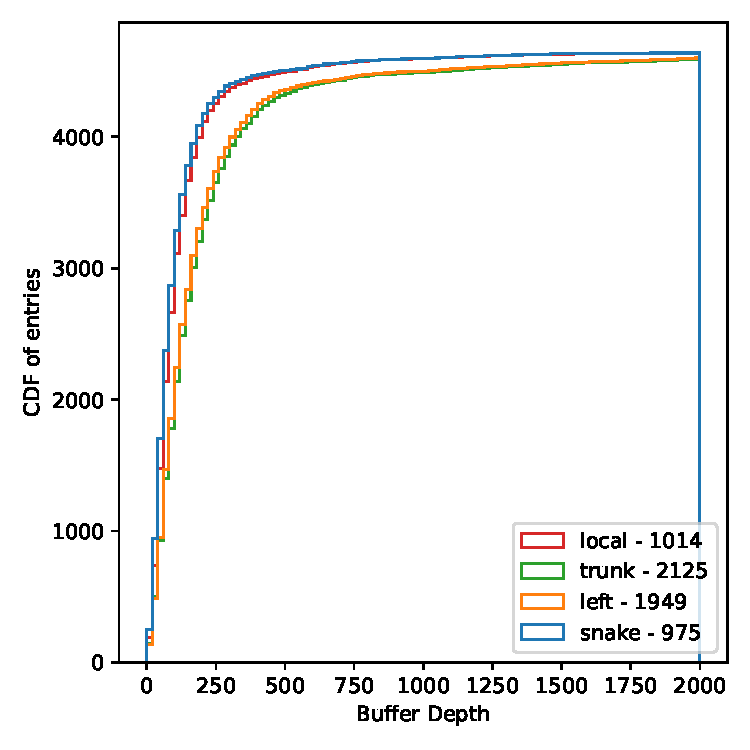
\includegraphics[width=\textwidth]{./images/example_16_remote_stack_slow.pdf}
      \caption[]%
      {{\small remote stack}}    
  \end{subfigure}
  \vskip\baselineskip
  \begin{subfigure}[b]{0.475\textwidth}   
      \centering 
      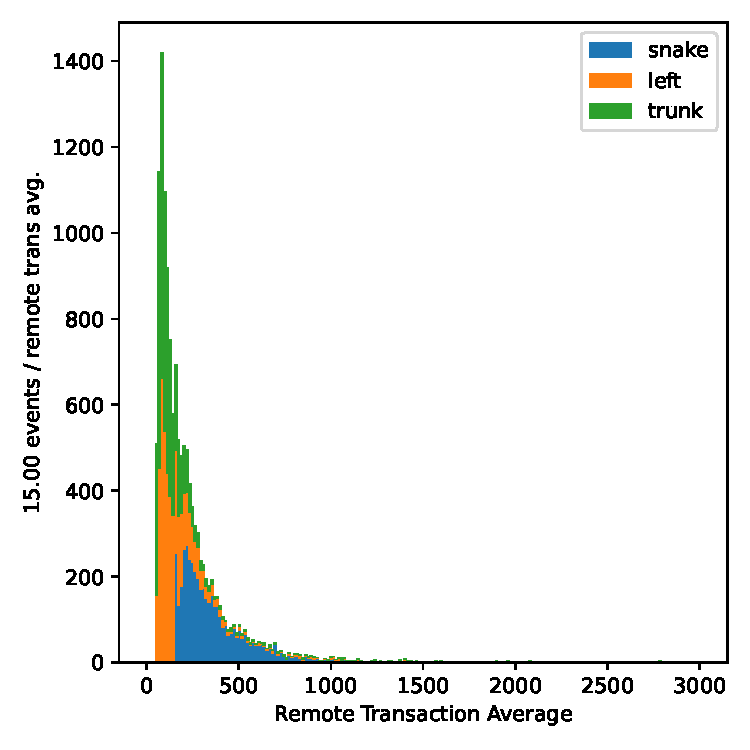
\includegraphics[width=\textwidth]{./images/example_16_remote_transact_slow.pdf}
      \caption[]%
      {{\small transact}}    
  \end{subfigure}
  \hfill
  \begin{subfigure}[b]{0.475\textwidth}   
      \centering 
      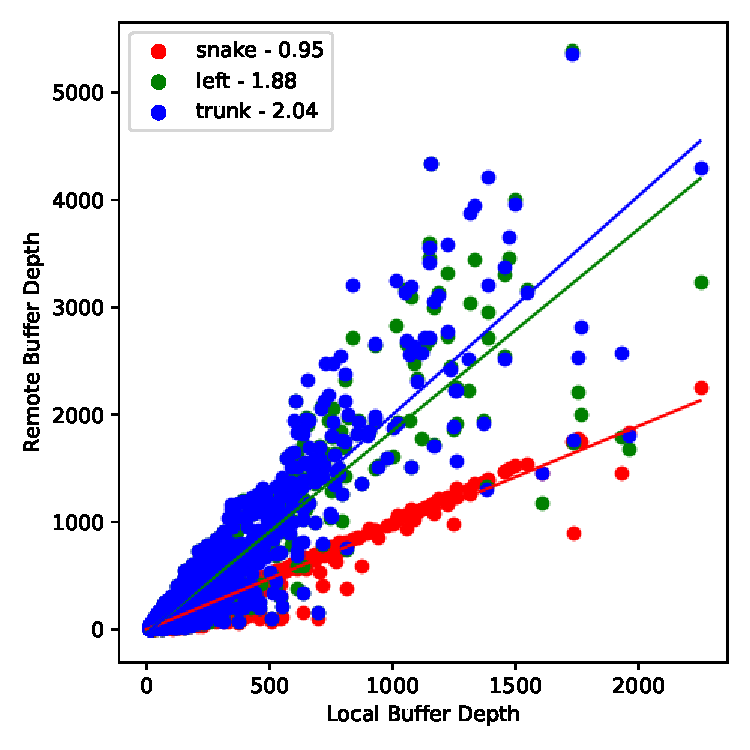
\includegraphics[width=\textwidth]{./images/example_16_route_fits_slow.pdf}
      \caption[]%
      {{\small route fits}}    
  \end{subfigure}
  \caption[ Information on the 4 by 4 tile. ]
  {\small all of the data } 
  \label{fig:example_plots_for_digital_sim}
\end{figure*}

%%% Example of Digital Simulation Reconstruction
\begin{figure*}
  \centering
  \begin{subfigure}[b]{0.475\textwidth}
      \centering
      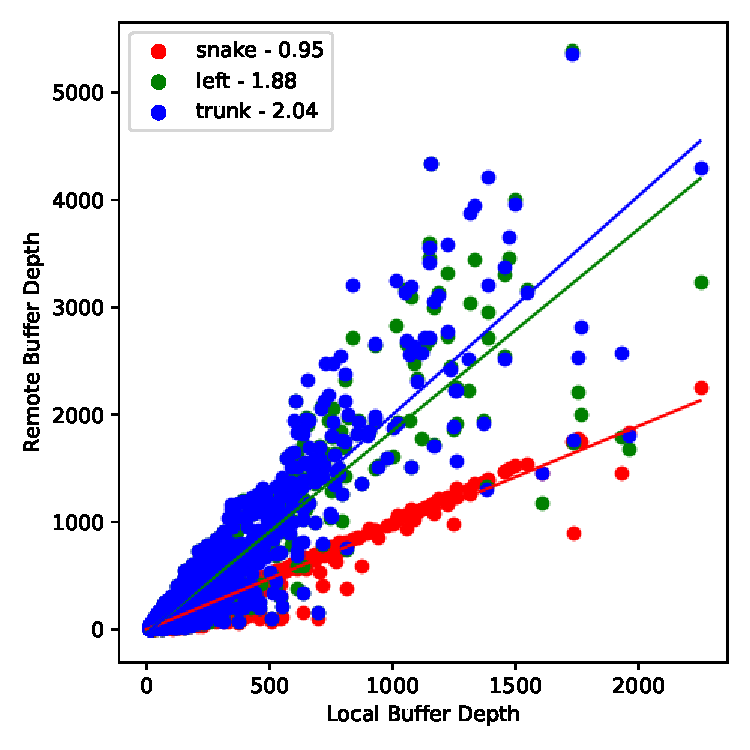
\includegraphics[width=\textwidth]{./images/example_16_route_fits_slow.pdf}
      \caption[]%
      {\small 16 Sized Tile}    
  \end{subfigure}
  \hfill
  \begin{subfigure}[b]{0.475\textwidth}  
      \centering 
      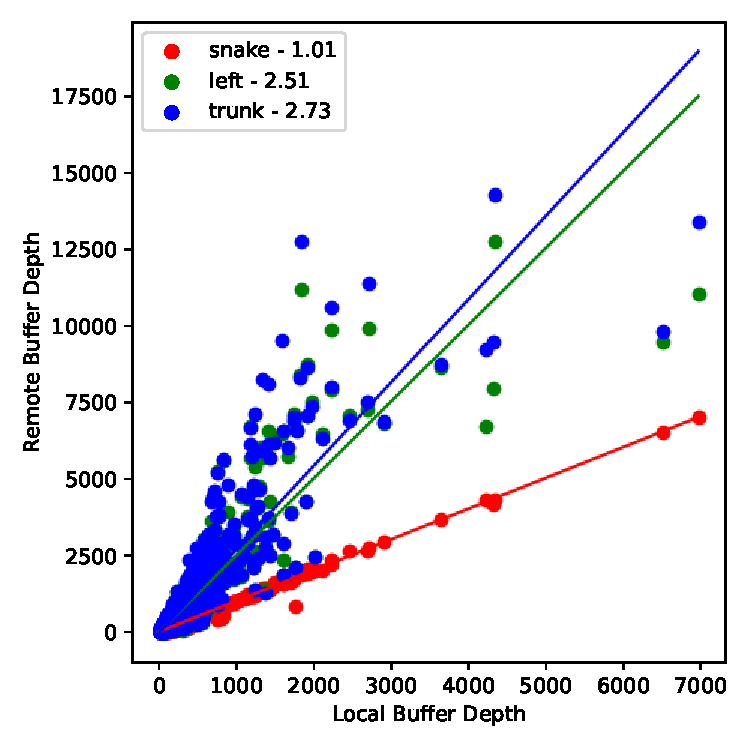
\includegraphics[width=\textwidth]{./images/example_64_route_fits_slow.pdf}
      \caption[]%
      {\small 64 Sized tile}    
  \end{subfigure}
  \vskip\baselineskip
  \begin{subfigure}[b]{0.475\textwidth}   
      \centering 
      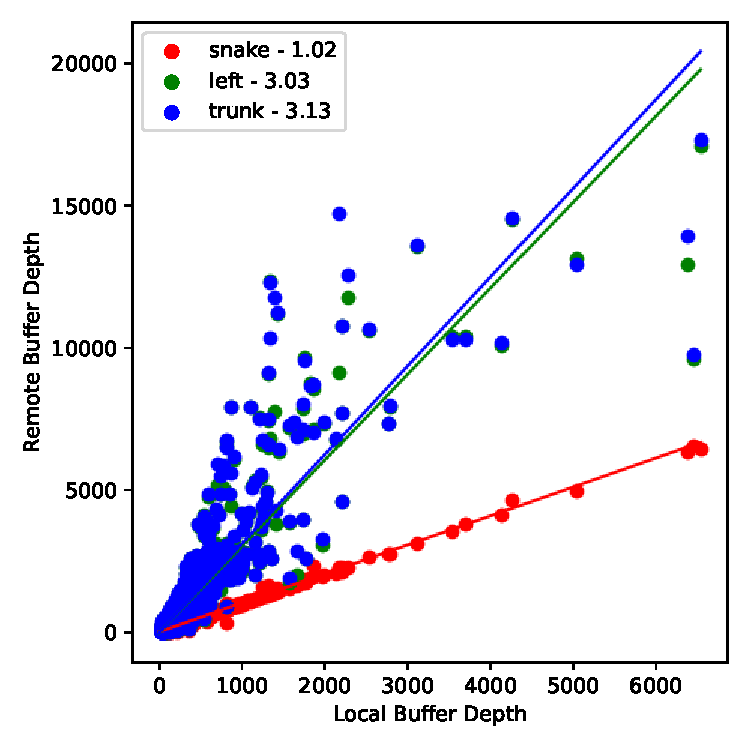
\includegraphics[width=\textwidth]{./images/example_140_route_fits_slow.pdf}
      \caption[]%
      {\small 140 Sized tile}    
  \end{subfigure}
  \hfill
  \begin{subfigure}[b]{0.475\textwidth}   
      \centering 
      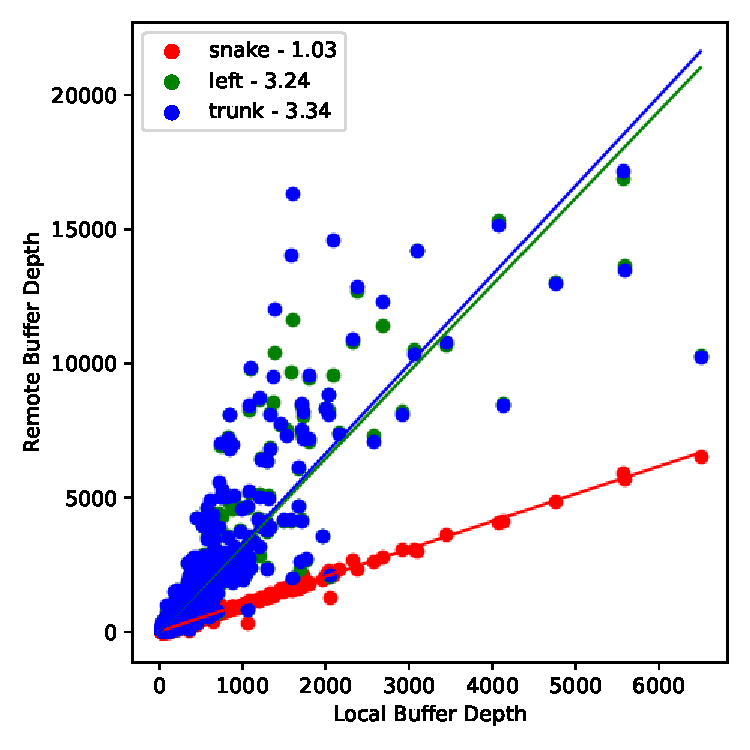
\includegraphics[width=\textwidth]{./images/example_256_route_fits_slow.pdf}
      \caption[]%
      {\small 256 Sized Tile}    
  \end{subfigure}
  \caption[ Information on the 4 by 4 tile. ]
  {\small all of the data } 
  \label{fig:compare_slow_plots_for_digital_sim_slow}
\end{figure*}

%%% Example of Digital Simulation Reconstruction
\begin{figure*}
  \centering
  \begin{subfigure}[b]{0.475\textwidth}
      \centering
      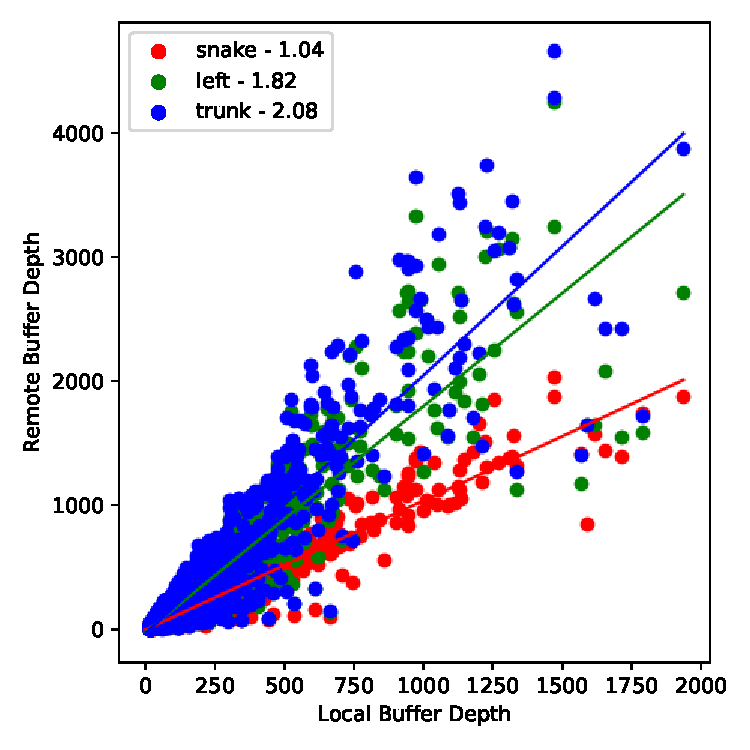
\includegraphics[width=\textwidth]{./images/example_16_route_fits.pdf}
      \caption[]%
      {\small 16 Sized Tile}    
  \end{subfigure}
  \hfill
  \begin{subfigure}[b]{0.475\textwidth}  
      \centering 
      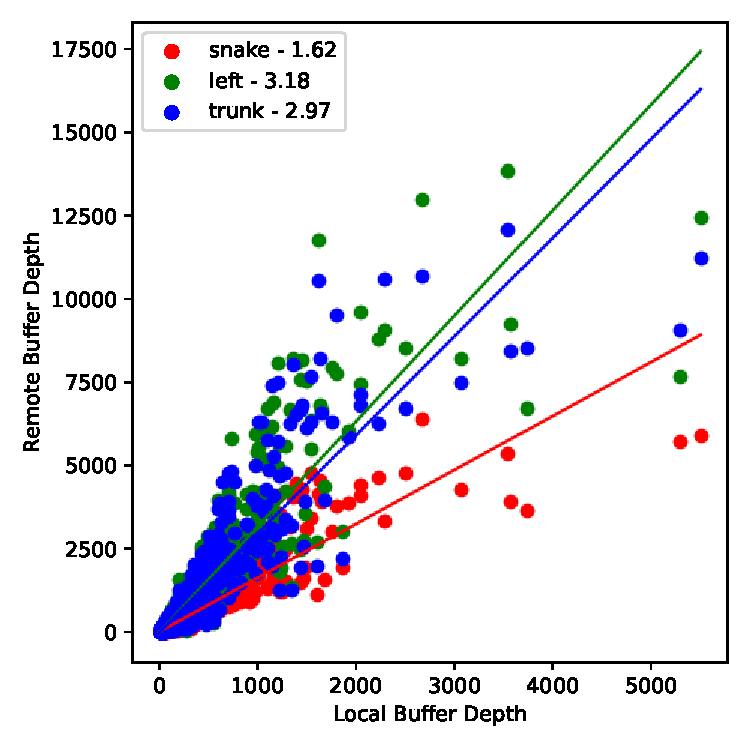
\includegraphics[width=\textwidth]{./images/example_64_route_fits.pdf}
      \caption[]%
      {\small 64 Sized tile}    
  \end{subfigure}
  \vskip\baselineskip
  \begin{subfigure}[b]{0.475\textwidth}   
      \centering 
      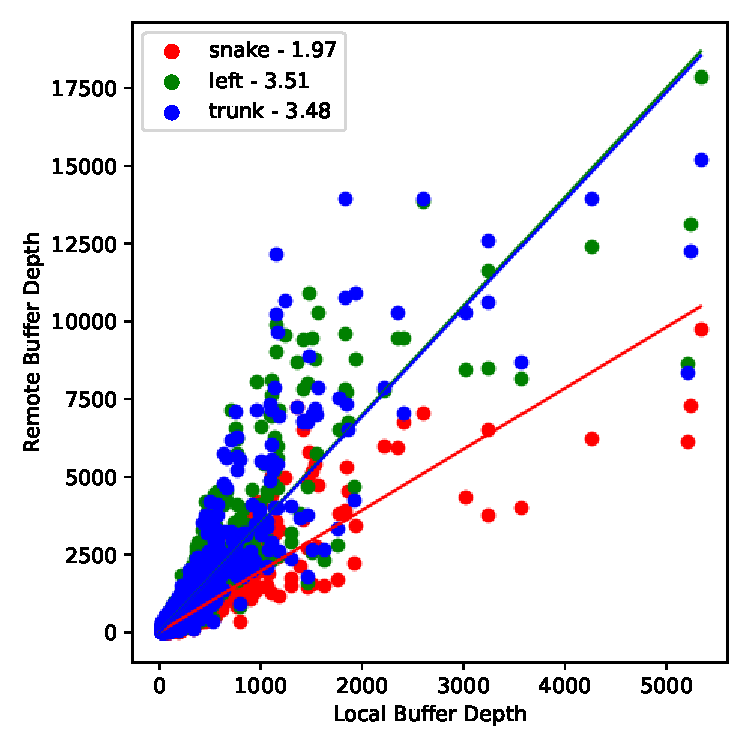
\includegraphics[width=\textwidth]{./images/example_140_route_fits.pdf}
      \caption[]%
      {\small 140 Sized tile}    
  \end{subfigure}
  \hfill
  \begin{subfigure}[b]{0.475\textwidth}   
      \centering 
      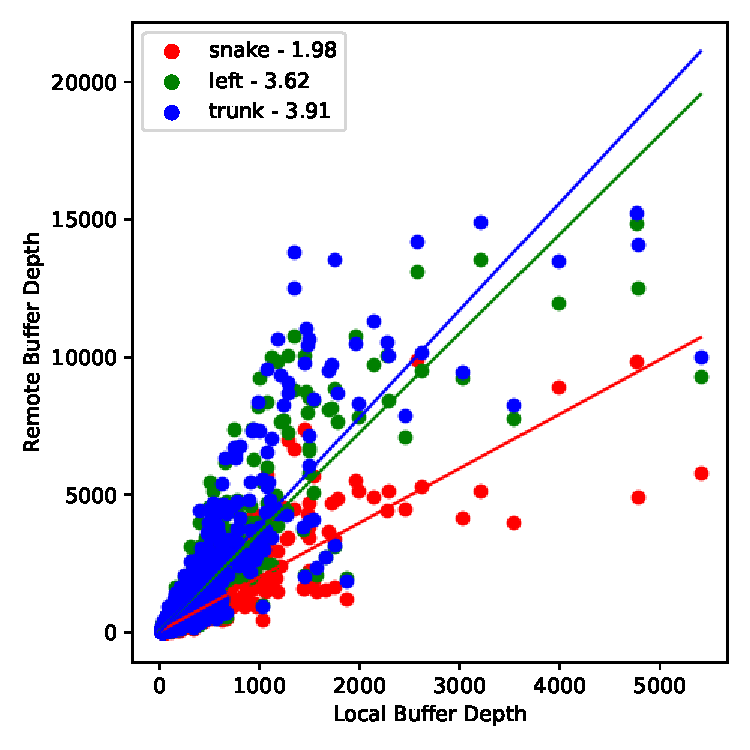
\includegraphics[width=\textwidth]{./images/example_256_route_fits.pdf}
      \caption[]%
      {\small 256 Sized Tile}    
  \end{subfigure}
  \caption[ Information on the 4 by 4 tile. ]
  {\small all of the data } 
  \label{fig:compare_fast_plots_for_digital_sim_slow}
\end{figure*}

%% table information
\begin{table}
	\begin{center}
		\begin{tabular}{|c|c|c|c|c|c|}
			\hline
			Freq. & Tile Size & Mean Local Hits & Snake & Left & Trunk \\
			\hline
			5\% & 16 & 48.250 & 423.293 & 166.403 & 138.380 \\
			\hline
			0.5\% & 16 & 51.846 & 449.861 & 177.357 & 147.346 \\
			\hline
			5\% & 64 & 34.129 & 1332.440 & 286.929 & 227.595 \\
			\hline
			0.5\% & 64 & 36.268 & 1400.794 & 301.775 & 239.087 \\
			\hline
			5\% & 140 & 26.521 & 2298.912 & 355.037 & 262.448 \\
			\hline
			0.5\% & 140 & 28.173 & 2416.778 & 373.173 & 275.614 \\
			\hline
			5\% & 256 & 24.343 & 4020.649 & 465.629 & 354.405 \\
			\hline
			0.5\% & 256 & 25.752 & 4209.196 & 487.090 & 370.695 \\
			\hline
		\end{tabular}
	\end{center}
	\caption{Transaction summary data is shown.
	The mean local hits column indicates the mean average of resets injected into the ASICs within the tile from an electron neutrino events.
	The Snake, Left, and Trunk, columns indicate the mean number of remote packet transactions which occured during the full 10 second simulation run.
	As expected, the amount of packet transactions in the snake routing scales with the tile size, whereas the Left and Trunk routings do not.
	The frequency distribution of the tiles does not affect the total number of transactions in the simulated event.
	These results can be used to indicate the amount of power and active time required for a tile to fully readout an electron neutrino event. 
	For example, if a tile size of 256 with a snake routing takes 4020 packets on average to digitize the event, then there are a total of slightly more than one million packets sent.
	If the amount of power used during single packet transaction is known, this ratio could be used to estimate the dissipated power during the back-end readout. 
	}
	\label{tab:transact}
\end{table}
\begin{table}
	\begin{center}
		\begin{tabular}{|c|c|c|l|r|l|r|l|r|}
			\hline
			Freq. & Tile Size & Local Hits & 95-S & 99-S & 95-L & 99-L & 95-T & 99-T \\
			\hline
			5\% & 16 & 939 & 320 & 1014 & 535 & 1736 & 607 & 1971 \\
			\hline
			0.5\% & 16 & 1014 & 322 & 975 & 603 & 1949 & 652 & 2125 \\
			\hline
			5\% & 64 & 1200 & 598 & 2191 & 1098 & 4394 & 975 & 4295 \\
			\hline
			0.5\% & 64 & 1307 & 403 & 1328 & 970 & 4298 & 974 & 4521 \\
			\hline
			5\% & 140 & 1182 & 852 & 3486 & 1455 & 6558 & 1343 & 6309 \\
			\hline
			0.5\% & 140 & 1393 & 440 & 1464 & 1327 & 6616 & 1382 & 6757 \\
			\hline
			5\% & 256 & 1456 & 1039 & 3637 & 2026 & 7679 & 2008 & 8250 \\
			\hline
			0.5\% & 256 & 1670 & 527 & 1668 & 1773 & 7460 & 1784 & 7368 \\
			\hline
		\end{tabular}
	\end{center}
	\caption{Buffer Data}
	\label{tab:buffers}
\end{table}
\begin{table}
	\begin{center}
		\begin{tabular}{|c c|c|c|c|c|}
			\hline
			Tile Size & Frequency & Snake & Left & Trunk & Push \\
			\hline
			16 & 0.5\% & 0.948 & 1.879 & 2.039 & 0.979 \\
			& 5\% & 1.041 & 1.823 & 2.082 & 1.031 \\
			\hline
			64 & 0.5\% & 1.006 & 2.514 & 2.727 & 0.999 \\
			& 5\% & 1.623 & 3.176 & 2.969 & 1.11 \\
			\hline
			140 & 0.5\% & 1.021 & 3.033 & 3.131 & na \\
			& 5\% & 1.966 & 3.506 & 3.481 & na \\
			\hline
			256 & 0.5\% & 1.027 & 3.243 & 3.336 & na \\
			& 5\% & 1.981 & 3.616 & 3.913 & na \\
			\hline
		\end{tabular}
	\end{center}
	\caption{Transaction fit summary results.
	The values shown from the fits indicate the linear fit to the results to predict the relationship between the local and remote FIFO depth requirements.
	Push fit data is not available for larger tiles (140 and 256) due to simulation time constraints.
	}
	\label{tab:fit}
\end{table}


\section{Summary and Further Studies}~\label{sec:further_studies}
